
\section{Leitungstheorie}

	\begin{tabular}{p{8cm}p{4.5cm}p{5cm}}
		\begin{minipage}{8cm}
	    	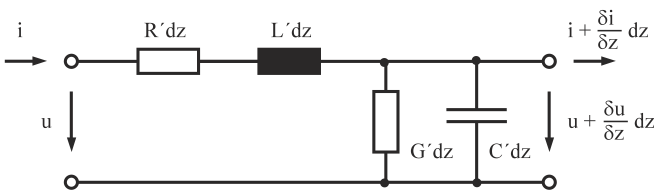
\includegraphics[width=8cm]{./bilder/LeitungselementESB.png}
	    \end{minipage}&
		\begin{minipage}{4.5cm}
	    	\textbf{Leitungsbeläge}\\
	    	$R'[\frac{\Omega}{m}]: \text{Widerstandsbelag}$\\
	    	$L'[\frac{H}{m}]: \text{Induktivitätsbelag}$\\
	    	$G'[\frac{S}{m}]: \text{Leitwertbelag}$\\
	    	$C'[\frac{F}{m}]: \text{Kapazitätsbelag}$\\
	    \end{minipage}&
		\begin{minipage}{5cm}
        	\textbf{Leitungsgleichungen:}\\
				\vspace{0.3cm}
        		$\dfrac{\partial i}{\partial z} = -G'u - C'\dfrac{\partial u}{\partial t}$\\
        		\vspace{0.3cm}
        		$\dfrac{\partial u}{\partial z} = -R'i - L'\dfrac{\partial i}{\partial t} $         		 	
        \end{minipage}\\
        \textbf{Leitung als Zweitor}&\\
		\begin{minipage}{8cm}
			$\underline{U}_1=\cosh(\underline{\gamma} l)\cdot \underline{U}_2+
			 \underline{Z}_0 \cdot \sinh(\underline{\gamma} l)\cdot \underline{I}_2$\\
			 $\underline{I}_1=\frac{1}{\underline{Z}_0}\cdot \sinh(\underline{\gamma} l)\cdot
			\underline{U}_2+ \cosh(\underline{\gamma} l)\cdot \underline{I}_2$ 	
        \end{minipage}
        &
        \begin{minipage}{9cm}
		$\begin{bmatrix}
          	\underline{U}_1\\
          	\underline{I}_1
          \end{bmatrix}=
		  \begin{bmatrix}
          	cosh(\underline{\gamma} l) & \underline{Z}_0 sinh(\underline{\gamma} l)\\
          	\frac{1}{\underline{Z}_0}sinh(\underline{\gamma} l) & cosh(\underline{\gamma} l)
          \end{bmatrix} \cdot
		  \begin{bmatrix}
          	\underline{U}_2\\
          	\underline{I}_2
          \end{bmatrix}$\\
        \end{minipage}\\
	\end{tabular}\\
		wenn $\alpha l >> \beta l$ kann $cosh(\underline{\gamma} l)\approx sinh(\underline{\gamma}
		l)=\frac{1}{2} e^{\underline{\gamma} l}$ angenommen werden!!!
	
	

	\subsection{Verlustbehaftete Leitungen}
		\renewcommand{\arraystretch}{1.7}
		\begin{tabular}{| p{6cm} | l |}
			\hline
				\textbf{Ausbreitungskonstante} $ \gamma = \left[\frac{1}{m}\right]$
				& $\underline{\gamma}=\alpha+j\beta=\sqrt{(R'+j\omega L')(G'+j\omega C')} = \sqrt{(R'G'-\omega^2L'C')+j\omega(R'C'+L'G')}$\\
			\hline
				\textbf{Dämpfungs-Belag} $\alpha =\left[\frac{Np}{m}\right]$
				& \textbf{Neper:} $1 Np=\frac{ln(10)}{20}dB$ \qquad $dB = Np \cdot \frac{20}{ln\left(10\right)}$\\
			\hline
				\textbf{Phasen-Belag} $\beta=\left[\frac{rad}{m}\right]$
				& $\beta=\frac{\omega}{v_{ph}}$\\
			\hline
				\textbf{Wellengleichung}
				& \parbox{10cm}{$\boxed{ \underline{U}(z) =\underline{U}_v+\underline{U}_r } =\underline{U}_{v0} \cdot e^{-\underline{\gamma} z} +
                   	\underline{U}_{r0} \cdot e^{\underline{\gamma}
                   	z}\\
                   	\boxed{\underline{I}(z)=\underline{I}_v-\underline{I}_r} = \underline{I}_{v0} \cdot e^{-\underline{\gamma} z} -
                   	\underline{I}_{r0} \cdot e^{\underline{\gamma}
                   	z}$ }\\
			\hline			
				\textbf{Wellenwiderstand}
				& $\underline{Z}_0 = \underline{Z}_W = \sqrt{\frac{R'+j\omega L'}{G'+j\omega C'}}$
				$=\sqrt{\underline{Z}_L \cdot \underline{Z}_K} =\frac{\underline{U}_v}{\underline{I}_v} =\frac{\underline{U}_r}{\underline{I}_r}$\\
			\hline
				\textbf{Vorlaufende Anfangsspannung}
				& $\underline{U}_{Av}$ sieht nur $\underline{Z}_0 \Rightarrow \underline{I}_{Av} = \frac{\underline{U_{Av}}}{\underline{Z}_0}$\quad U-Quelle am Eingang: $\underline{U}_{Av} = \underline{U}_q\frac{\underline{Z}_0}{R_i+\underline{Z}_0}$\\
			\hline
				\textbf{Phasengeschw., Wellenlänge}
				& $v_{ph}=\frac{\lambda}{T} = \frac{\omega}{\beta} = \lambda \cdot f 
				\qquad \lambda=\frac{2\pi}{\beta}=\frac{v_{ph}}{f}$ \\
			\hline
				\textbf{Freiraumwellenlänge}
				& $\lambda_0=\frac{c}{f}=\frac{2\pi c}{\omega} \qquad c\approx 3\cdot10^8 \frac{m}{s}$\\
			\hline
		\end{tabular}	
		\subsubsection{Beschaltete Leitung}
		\begin{tabular}{| p{6cm} | l |}
			\hline
				\textbf{Reflexionskoeffizienten} &
				$r = \frac{\underline{U}_{r}}{\underline{U}_{v}}= \frac{\underline{I}_{r}}{\underline{I}_{v}} = \frac{\underline{Z}-\underline{Z}_0}
				{\underline{Z}+\underline{Z}_0}\qquad$\par 
				\parbox[c][1.75cm]{5cm}{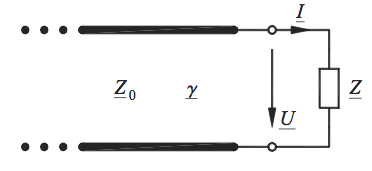
\includegraphics[height = 1.5cm]{./bilder/Beschaltete_Leitung}}
				\\
				\hfill Am Anfang: & $\underline{r}_{A}= \underline{r}_{E}\cdot e^{-2\gamma l}=\frac{\underline{U}_{Ar}}{\underline{U}_{Av}}=\frac{\underline{Z}_{A}-\underline{Z}_0}
				{\underline{Z}_{A}+\underline{Z}_0}$ \\
				\hfill Am Ende:	&
				$\underline{r}_{E}=\frac{\underline{U}_{Er}}{\underline{U}_{Ev}}=\frac{\underline{Z}_{E}-\underline{Z}_0}
				{\underline{Z}_{E}+\underline{Z}_0}$\\
			\hline
			  	\textbf{$\underline{Z}$ beim Reflexionsfaktor $\underline{r}$}
			  	& $\underline{Z}=\underline{Z}_0 \cdot \frac{1+\underline{r}}{1-\underline{r}}$\\
			\hline
				\textbf{Spannungen / Ströme}
				& $\underline{U}_r = \underline{r} \cdot \underline{U}_v \Leftrightarrow \underline{I}_r = \underline{r} \cdot \underline{I}_v
				\qquad \underline{U} = \underline{U}_v(1+r)
				\qquad \underline{U} = \underline{U}_r(1+\frac{1}{r}) $\\
			\hline
				\textbf{Transformations-Eigenschaften}
				& \parbox{3cm}{
				 $\underline{U}_{Ev} = \underline{U}_{Av}\cdot e^{-\underline{\gamma}\cdot l}$\\
				 $\underline{U}_{Ar} = \underline{U}_{Er}\cdot e^{-\underline{\gamma}\cdot l}$}
				 \hspace{0.5cm}\parbox[c][2cm]{8cm}{
				 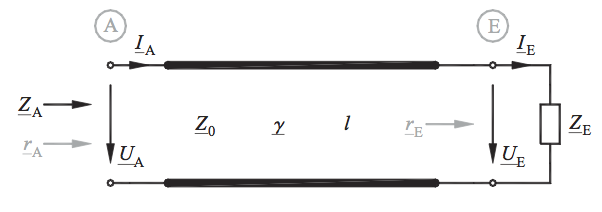
\includegraphics[height = 1.75cm]{./bilder/Leitungstransformation}}
				 
				 \\	
				\hfill von $\underline{r}$: & $\underline{r}_{A}= \underline{r}_{E}\cdot e^{-2\gamma l}$\\
				\hfill von $\underline{Z}$:	& $\underline{Z}_A = \underline{Z}_0 \cdot \frac{1+\underline{r}_A}{1-\underline{r}_A} = \underline{Z}_0
				\frac{\underline{Z}_0 \cdot \sinh \underline{\gamma}l +\underline{Z}_E \cdot \cosh\underline{\gamma}l} {\underline{Z}_0 \cdot \cosh \underline{\gamma}l+\underline{Z}_E \cdot \sinh\underline{\gamma}l} = 				\underline{Z}_0
				\frac{\underline{Z}_E+\underline{Z}_0 \cdot \tanh\underline{\gamma}l}{\underline{Z}_0+\underline{Z}_E \cdot \tanh\underline{\gamma}l}
				$\\
			\cline{2-2}			
				\hfill Keine Reflektion:
				& $\underline{Z}_{E}=\underline{Z}_0$ , $\underline{r}_E = 0 \quad \rightarrow \quad \underline{Z}_{A}=\underline{Z}_0$ ,  $\underline{r}_A = 0$\\
				\hfill Kurzschluss:
				& $ \underline{Z}_{E} = 0$ , $\underline{r}_E = -1 \quad \rightarrow \quad \underline{Z}_{A} = \underline{Z}_{K} = \underline{Z}_0 \frac{\sinh \underline{\gamma}l}{\cosh \underline{\gamma}l}$
					\\
				\hfill Leerlauf:
				&$ \underline{Z}_{E} \rightarrow \infty$ , $\underline{r}_E = +1 \quad \rightarrow \quad \underline{Z}_{A} = \underline{Z}_{L} = \underline{Z}_0 \frac{\cosh \underline{\gamma}l}{\sinh \underline{\gamma}l}$\\
			\hline  
%			  \textbf{Reflexionsdämpfung / Dämpfungsverlust}
%			  & $a=-\ln|\underline{r}|\text{ Neper}=-20\cdot \log|\underline{r}|\text{dB} \quad \quad A = -10\log(\frac{P_L}{P_{max}})$\\
%			\hline
%				\textbf{Bei Abschluss mit $\underline{Z}_W$} &
%				$\underline{U}_1(z) = \underline{U}_2\cdot e^{\gamma z} \qquad
%				\underline{I}_1(z) =- \underline{I}_2\cdot e^{\gamma z} \qquad \alpha l =
%				ln(\frac{U1}{U2}) \qquad \beta l = arg(\frac{\underline{U}_1}{\underline{U}_2})$\\
%			\hline
			 
%				\textbf{wichtige Formeln}&
%				$\gamma l=\frac{1}{2}ln(\frac{1+\sqrt{\underline{Z}_K/\underline{Z}_L}}{1-
%				\sqrt{\underline{Z}_K/\underline{Z}_L}})$ \qquad
%				$\sqrt{\frac{\underline{Z}_K}{\underline{Z}_L}}=\frac{e^{2\gamma
%				L}-1}{e^{2\gamma K}+1}$ \qquad $e^{2\gamma l}=e^{2\alpha l} \cdot e^{j2\beta
%				l}=\frac{1+\sqrt{{\underline{Z}_K}/
%				{\underline{Z}_L}}}{1-\sqrt{{\underline{Z}_K}/ {\underline{Z}_L}}}$\\
%			\hline
		\end{tabular}
	\renewcommand{\arraystretch}{1}
	
	
	\subsection{Verlustfreie Leitungen}
		\renewcommand{\arraystretch}{1.5}
		\begin{tabular}{| l | c | c |}
			\hline
				\textbf{Fortpflanzungskonstante}
				& $\gamma=j\beta=j\omega \sqrt{L'C'} $
				&\\
			\hline
				\textbf{Dämpfungsmass}
				& $R'=G'=0\quad \Rightarrow \quad \alpha=0$
				&\\
			\hline
				\textbf{Phasenmass}
				& $\beta=\omega\sqrt{L'C'}$
				& $[\beta] = \frac{rad}{m}$\\
			\hline
				\textbf{Wellenwiderstand}
				& $Z_0 = R_0 =\sqrt{\frac{L'}{C'}}$, rein reel!
				& $[Z_0] = \Omega$\\
			\hline
				\textbf{Verkürzungsfaktor}
				& $ VK = \frac{\lambda}{\lambda_0}=\frac{v_{ph}}{c} \qquad v_{ph} = \frac{1}{\sqrt{L'C'}}$ &\\
				\hfill Koaxialkabel:& $v_{ph} = \frac{c}{\sqrt{\varepsilon_r \cdot \mu_r}}  \underbrace{=}_{\mu_r = 1} \frac{c}{\sqrt{\epsilon_r}} \quad \Rightarrow \quad VK = \frac{1}{\sqrt{\varepsilon_r \cdot \mu_r}} \underbrace{=}_{\mu_r = 1} \frac{1}{\sqrt{\varepsilon_r}} $ & \\ 
			\hline
				\textbf{Transformation}
				& $\underline{Z}_A=R_0\frac{\underline{Z}_{E}+jR_0\tan(\beta l)}{R_0+j\underline{Z}_{E}\tan(\beta l)}$
				&\\
				& $\underline{r}_A=\underline{r}_E\cdot e^{-2j\beta l}$
				&\\
			\cline{2-3}
				\hfill Leerlauf: $ \underline{r}_E=+1$
				& $\underline{Z}_A=-j\frac{R_0}{\tan(\beta l)}$
				&\\
				\hfill Kurzschluss $ \underline{r}_E=-1$
				& $\underline{Z}_A=j R_0 \tan(\beta l)$
				&\\
			\hline
%				$\begin{matrix}
%					\textbf{LE mit }\underline{Z}_{Last} \textbf{ abgeschlossen}\\
%					%\underline{Z}_L=\underline{Z}_W \quad \underline{\Gamma}=0
%				\end{matrix}$
%				& $\begin{matrix}
%                  	\frac{\underline{U}_1}{\underline{I}_2}=\cosh(j\beta
%                  	l)\underline{Z}_{Last}+\underline{Z}_W \sinh(j\beta l)\\
%                  	\frac{\underline{I}_1}{\underline{I}_2}=\frac{1}{\underline{Z}_W} \sinh(j\beta
%                  	l)\underline{Z}_{Last}+ \cosh(j\beta l) \end{matrix}$
%                &\\
%                \hline
                 \textbf{Leistungen}
                 &
                 $P_r= \frac{U^2_{Ar}}{R_0}=\frac{r_A^2U^2_{Av}}{R_0}=r_A^2 P_v$\qquad
                 $P_{E}=P_v(1-r_A^2)$ & \\
                 & $P_v = U_{Av} \cdot               I_{Av} = \frac{U^2_{Av}}{R_0}$ = z.B. Antennenleistung &\\
             \hline
		\end{tabular}
	\renewcommand{\arraystretch}{1}
%	\newpage
% 	\subsubsection{Leitungen in Vierpolnotation}
% 	\renewcommand{\arraystretch}{1.1}
% 		\begin{tabular}{| l | c |}
% 			\hline
% 				\textbf{A Matrix}
% 				& $\begin{bmatrix}
%                   	\underline{U}_1\\
%                   	\underline{I}_1
%                   \end{bmatrix}=
% 				  \begin{bmatrix}
%                   	cosh(\gamma l) & \underline{Z}_W sinh(\gamma l)\\
%                   	\frac{1}{\underline{Z}_W}sinh(\gamma l) & cosh(\gamma l)
%                   \end{bmatrix} \cdot
% 				  \begin{bmatrix}
%                   	\underline{U}_2\\
%                   	\underline{I}_2
%                   \end{bmatrix}$\\
% 			\hline
% 				\textbf{T-Ersatz}
% 				& $\underline{Z}_1=tanh(\frac{\gamma l}{2})\underline{Z}_W=\underline{Z}_2$\\
% 			\hline
% 				\textbf{Pi-Ersatz}
% 				& $\underline{Z}_1=\frac{\underline{Z}_W}{tanh(\frac{\gamma l}{2})}=\underline{Z}_2$\\
% 			\hline
% 		\end{tabular}
% 	\renewcommand{\arraystretch}{1}


\subsubsection{Stehwellenverhältnis und Anpassfaktor}
  \renewcommand{\arraystretch}{1.3}
   \begin{tabular}{|l|l|}
   	 \hline
   		Grundlagen 
   		& $\underline{r}_E = r_E \cdot e^{j\varphi_E}$\\
   		& $l$ vom Ende weg gemessen!\\
   	  \hline
   		\textbf{Maximale Spannung}
   		& $U(l)_{max}$, wenn $\underline{U}_v$ und $\underline{U}_r$ in Phase $ \rightarrow l_{Umax} = \frac{\varphi_E}{2\beta} $\\
		\textbf{Minimale Spannung}
   		& $U(l)_{min}$, wenn $\underline{U}_v$ und $\underline{U}_r$ in Gegenphase $ \rightarrow l_{Umin} = \frac{\varphi_E \pm \pi}{2\beta} $\\   		
   	 \hline
   		\textbf{Stehwellenverhältnis} 
        & $VSWR = s = \frac{U_{max}}{U_{min}} = \frac{U_v + U_r}{U_v - U_r} = \frac{1 + r_E}{1-r_E}$\\
     \hline
     	\textbf{Anpassfaktor}
     	& $m = \frac{1}{s} = \frac{1 - r_E}{1+r_E}$\\
     \hline
     	empirische Ermittlung von $\underline{r}_E$ 
     	& $r_E = \frac{s - 1}{s+1} = \frac{1 - m}{1+m}$\\
     	& $\varphi_E = l_{Umax} \cdot 2 \beta$\\
     \hline
   \end{tabular}
  \renewcommand{\arraystretch}{1}
  
  
%\subsection{Kapazitätsbelag}
%	\begin{tabular}{ll}
%    	\begin{minipage}{12cm}
%			\renewcommand{\arraystretch}{1.1}
%				\begin{tabular}{| l | l |}
%					\hline
%						\textbf{Leiterpotential}
%						& $\vec{E}=-grad V$ \qquad $V(\varrho)=-\frac{\lambda}{\varepsilon_02\pi}ln\frac{\varrho}{k}$\\
%					\hline
%						\textbf{$\varrho$}
%						& $\begin{matrix}
%                           		\text{Abstand zwischen Linienladungen}\\
%                           		\text{und deren Spiegelungen}
%                           \end{matrix}$\\
%					\hline
%						\textbf{$k$}
%						& Integrationskonstante (kürzt sich weg)\\
%					\hline
%						\textbf{$\varepsilon_0$}
%						& $8,85419 \cdot 10^{-12} [\frac{As}{Vs}]$\\
%					\hline
%						$\begin{matrix}
%                         	\textbf{Leiterpotentiale}\\
%                         	(aus Beispiel)
%                         \end{matrix}$
%						& $\begin{matrix}
%                          	V_1=\frac{\lambda_1}{2\pi\varepsilon_0}(-ln\frac{r}{k}+ln\frac{2a}{k})+\frac{\lambda_2}{2\pi\varepsilon_0}(-ln\frac{\varrho_1}{k}+ln\frac{\varrho_2}{k})\\
%                          	V_2=\frac{\lambda_1}{2\pi\varepsilon_0}(-ln\frac{\varrho_1}{k}+ln\frac{\varrho_2}{k})+\frac{\lambda_2}{2\pi\varepsilon_0}(-ln\frac{r}{k}+ln\frac{2b}{k})
%                          \end{matrix}$\\
%					\hline
%						\textbf{Matrix Potentialkoeff.}
%						& $ \begin{bmatrix}
%								V_1 \\
%								V_2 \\
%							\end{bmatrix}=
%							\begin{bmatrix}
%								p_1 & p_0 \\
%								p_0 & p_2 \\
%							\end{bmatrix} \cdot
%							\begin{bmatrix}
%								\lambda_1 \\
%								\lambda_2 \\
%							\end{bmatrix}$\\
%					%\hline
%						\textbf{}
%						& $p_1=\frac{1}{2\pi \varepsilon_0}ln\frac{2a}{r}$ \quad
%						  $p_2=\frac{1}{2\pi \varepsilon_0}ln\frac{2b}{r}$ \quad
%				          $p_0=\frac{1}{2\pi \varepsilon_0}ln\frac{\varrho_1}{\varrho_2}$\\
%					\hline
%						\textbf{Matrix Kapazitätskoeff.}
%						& $ \begin{bmatrix}
%								\lambda_1 \\
%								\lambda_2 \\
%							\end{bmatrix}=
%							\begin{bmatrix}
%								C_1 & C_0 \\
%								C_0 & C_2 \\
%							\end{bmatrix} \cdot
%							\begin{bmatrix}
%								V_1 \\
%								V_2 \\
%							\end{bmatrix}$\\
%					%\hline
%						\textbf{}
%						& $C_1=\frac{p_2}{det\quad p}$ \quad
%						  $C_2=\frac{p_1}{det\quad p}$ \quad
%						  $C_0=\frac{p_0}{det\quad p}=C_{12}$\\
%						  &$C_{10}=C_1-C_0; C_{20}=C_2-C_0$\\
%					\hline
%				\end{tabular}
%			\renewcommand{\arraystretch}{1}
%		\end{minipage}
%    \end{tabular}
%	\begin{minipage}{6cm}
%    	\begin{tabular}{ll}
%	    	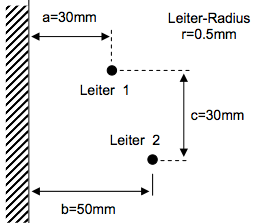
\includegraphics[width=3cm]{./bilder/LeitungenParallel.png}
%			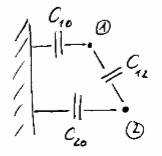
\includegraphics[width=3cm]{./bilder/LeitungenKapazitaeten.png} \\
%			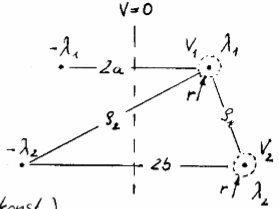
\includegraphics[width=5cm]{./bilder/LeitungenParallel2.png}
%		\end{tabular}
%	\end{minipage}
% 
%		
%\subsection{Induktivitätsbelag}
%	\begin{tabular}{ll}
%    	\begin{minipage}{12cm}
%			\renewcommand{\arraystretch}{1.1}
%				\begin{tabular}{| l | l |}
%					\hline
%						\textbf{Rotation B-Feld}
%						& $\vec{B}=rot\vec{A}$ \qquad $A(\varrho)=-\frac{\mu_0 I}{2\pi}ln(\frac{\varrho}{k})$\\
%					\hline
%						\textbf{Linienströme}
%						& $+I \qquad -I$\\
%					\hline
%						\textbf{$\mu_0$}
%						& $4\pi\cdot 10^{-7}[\frac{Vs}{Am}]$\\
%					\hline
%						$\begin{matrix}
%                         	\textbf{Leiterpotentiale}\\
%                         	(aus Beispiel)
%                         \end{matrix}$
%						& $\begin{matrix}
%                           	A^{+}=\frac{\mu_0 I}{2\pi}(-ln\frac{r}{k}+ln\frac{\varrho_1}{k}-ln\frac{2a}{k}+ln\frac{\varrho_2}{k})=\frac{\mu_0 I}{2\pi}ln\frac{\varrho_1\varrho_2}{2ar}\\
%                           	A^{-}=\frac{\mu_0 I}{2\pi}(-ln\frac{\varrho_1}{k}+ln\frac{r}{k}-ln\frac{\varrho_2}{k}+ln\frac{2b}{k})=-\frac{\mu_0 I}{2\pi}ln\frac{\varrho_1\varrho_2}{2br}
%                           \end{matrix}$\\
%					\hline
%						\textbf{Äussere Induktivität}
%						& $L_a=\frac{1}{I}(A^{+}-A^{-})=\frac{\mu_0}{2\pi}ln(\frac{\varrho_1^2 \varrho_2^2}{4r^2ab})$\\
%					\hline
%						\textbf{Innere Induktivität}
%						& $L_i=\frac{\mu_0}{8\pi} \quad \text{pro Leiter}$\\
%					\hline
%						\textbf{Induktivitätsbelag}
%						& $L'=L_a+2L_i=\frac{\mu_0}{\pi} (ln(\frac{\varrho_1 \varrho_2}{2r\sqrt{ab}})+\frac{1}{4})$\\
%					\hline
%				\end{tabular}
%			\renewcommand{\arraystretch}{1}
%		\end{minipage}
%    \end{tabular}
%	\begin{minipage}{6cm}
%    	\begin{tabular}{ll}
%	    	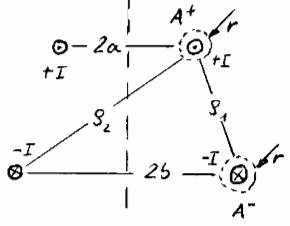
\includegraphics[width=5cm]{./bilder/Induktivitaetsbelag.png}
%		\end{tabular}
%	\end{minipage}
%
%\subsection{Stehende Wellen}
%%	\subsubsection{Eigenschaften}
%		\begin{tabular}{ll}
%	    	\begin{minipage}{9cm}
%				\renewcommand{\arraystretch}{1.1}
%					\begin{tabular}{| l | l |}
%						\hline
%							\textbf{Spannung}
%							& $|\underline{U}(z)|=|\underline{U}^+ e^{-j\beta z}(1+\underline{\Gamma}_L e^{2j\beta z})|=|\underline{U}^+| |1+\underline{\Gamma}_L e^{2j\beta z}|=|\underline{U}^+||1+|\underline{\Gamma}_L| e^{j(\Phi-2\beta z)}|$\\
%						\hline
%							\textbf{Strom}
%							& $|\underline{I}(z)|=|\underline{U}^+ / \underline{Z}||1-|\underline{\Gamma}_L| e^{j(\Phi-2\beta z)}|$\\
%						\hline
%							\textbf{Spannungsmaxima bei:}
%							& $e^{j(\Phi-2\beta z)}=1$\\
%						\hline
%							\textbf{Spannungsminima bei:}
%							& $e^{j(\Phi-2\beta z)}=-1$\\
%						\hline
%					\end{tabular}
%				\renewcommand{\arraystretch}{1}
%			\end{minipage}
%	    \end{tabular}
%
%		\begin{tabular}{p{9cm}p{9cm}}
%        	\begin{minipage}{8cm}
%            	Spannungsbetrag mit kompl. Abschlussimpedanz:\\
%            	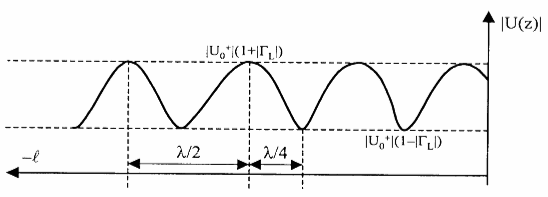
\includegraphics[height=2cm]{./bilder/VerlaufSpannungsbetrag.png}
%            \end{minipage}
%			&
%			\begin{minipage}{8cm}
%            	Spannungs- Strombetrag der offenen Leitung:\\
%            	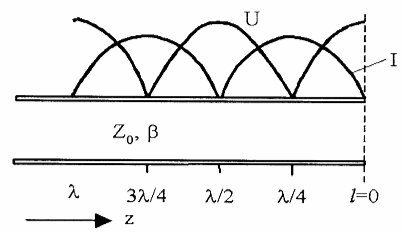
\includegraphics[height=2cm]{./bilder/VerlaufSpannungsbetragOffeneLtg.png}
%            \end{minipage}
%        \end{tabular}
%	
	\subsubsection{Spezialfälle}
		\textbf{Kurzschluss/Leerlauf}\\
			Bei Kurzschluss oder Leerlauf verschwinden die Spannungs- Stromminima.
			Da die rückläufige Welle eben soviel Energie transportiert wie die hinlaufende, wird längs der Leitung keine Energie transportiert.
			Es sieht so aus, als ob die Welle am Ort stehen bleibt.\\
		\textbf{Leitung ideal abgeschlossen}\\
			Ist die Leitung ideal abgeschlossen, existiert keine reflektierende Welle.
			Die hinlaufende Welle transportiert so die gesamte Energie vom Sender zum Empfänger.\\
		\textbf{Leitung nicht ideal abgeschlossen}\\
			Es entsteht beim Empfänger eine Überlagerung der absorbierten und der stehenden Welle.
			Aus dem Verhältnis von Spannungsmaximum zu Spannungsminimum entsteht das Stehwellenverhältnis VSWR.
			
\subsubsection{Beispiele zu Leitungsabschlüssen}
		\renewcommand{\arraystretch}{1.1}
		\begin{tabular}{| p{0.14\linewidth} | p{0.14\linewidth}  | p{0.14\linewidth}  | p{0.14\linewidth}  | p{0.14\linewidth}  | p{0.14\linewidth}  |}
			\hline
				\textbf{Fall}
				& 1
				& 2 
				& 3
				& 4
				& 5 \\
			\hline
				\textbf{Leitungsende}
				& Anpassung
				& Leerlauf: \newline Spannungs-\newline maximum
				& Kurzschluss: \newline Spannungs-\newline minimum
				& $\lambda/8$ Stichleit. KS
				& $\lambda/8$ Stichleit. LL \\
			\hline
				\textbf{SWR}
				& 1
				& $\infty$
				& $\infty$
				& $\infty$
				& $\infty$ \\
			\hline
				\textbf{$\underline{r}$}
				& $0$
				& $1 \angle 0 ^\circ$
				& $1 \angle 180 ^\circ$
				& $1 \angle 90 ^\circ$
				& $1 \angle 90 ^\circ$\\
			\hline
				\textbf{z}
				& $1+j0$
				& $\infty+j\infty$
				& $0+j0$
				& $0+j1$
				& $0-j1$ \\
			\hline
				\textbf{$v_{xm}$}
				& $-$
				& $\lambda/4$
				& $\lambda/2$
				& $3\lambda/8$
				& $\lambda/8$ \\
			\hline
				\textbf{Grafik}
				& 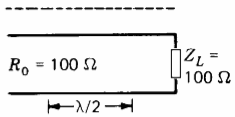
\includegraphics[height=0.9cm]{./bilder/Fall1.png}
				& 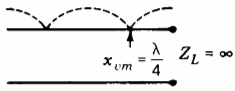
\includegraphics[height=0.9cm]{./bilder/Fall2.png}
				& 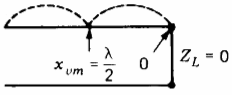
\includegraphics[height=0.9cm]{./bilder/Fall3.png}
				& 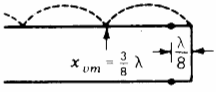
\includegraphics[height=0.9cm]{./bilder/Fall4.png}
				& 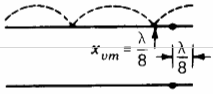
\includegraphics[height=0.9cm]{./bilder/Fall5.png} \\
			\hline
		\end{tabular}

%	\subsection{Mehrfachreflexion}
%% 	\textbf{Lastseitig falsch abgeschlossen}\\
%% 	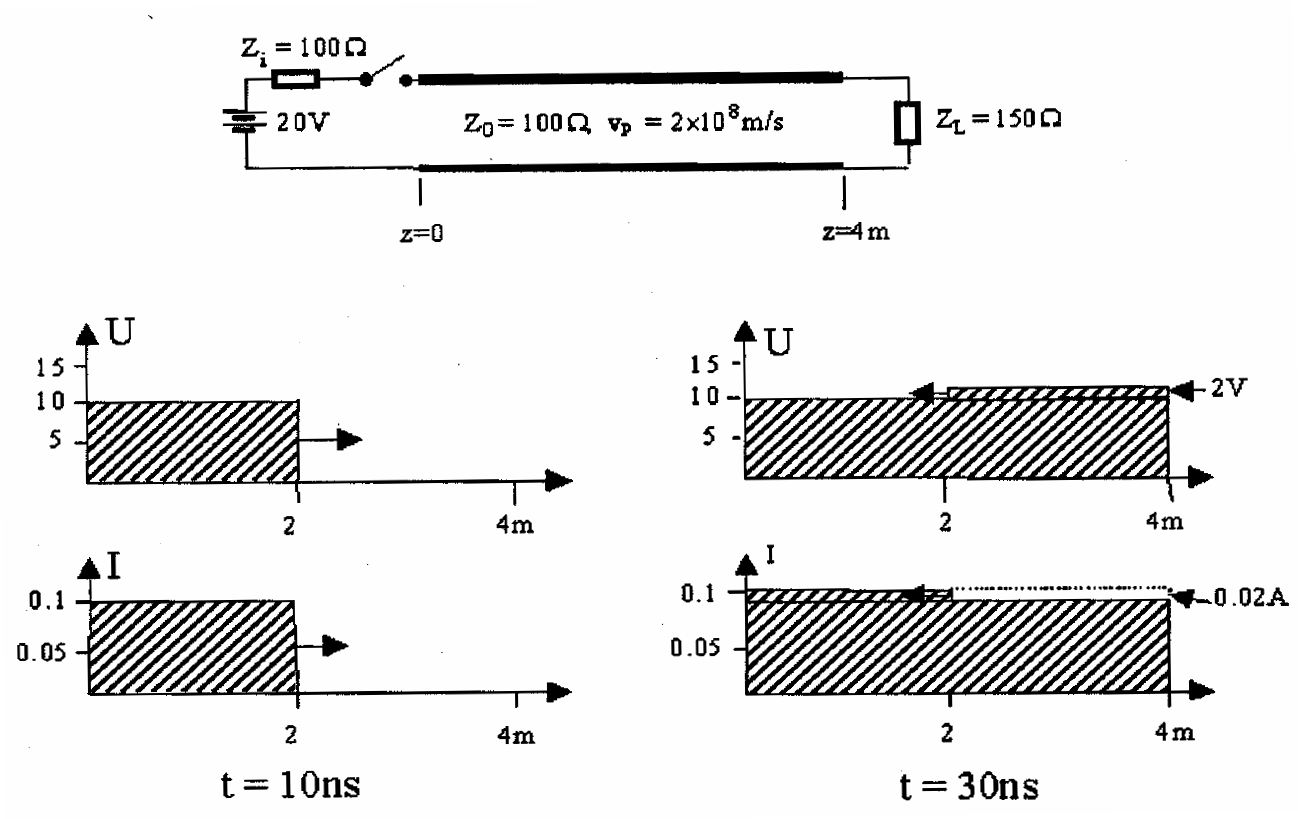
\includegraphics[height=3.5cm]{../El4/bilder/Leitungen_MFReflx_EnAP_SAP.png} \textbf{text folgt} \\
%	\begin{tabular}{p{9cm}p{9cm}}
%		\begin{minipage}{8cm}
%			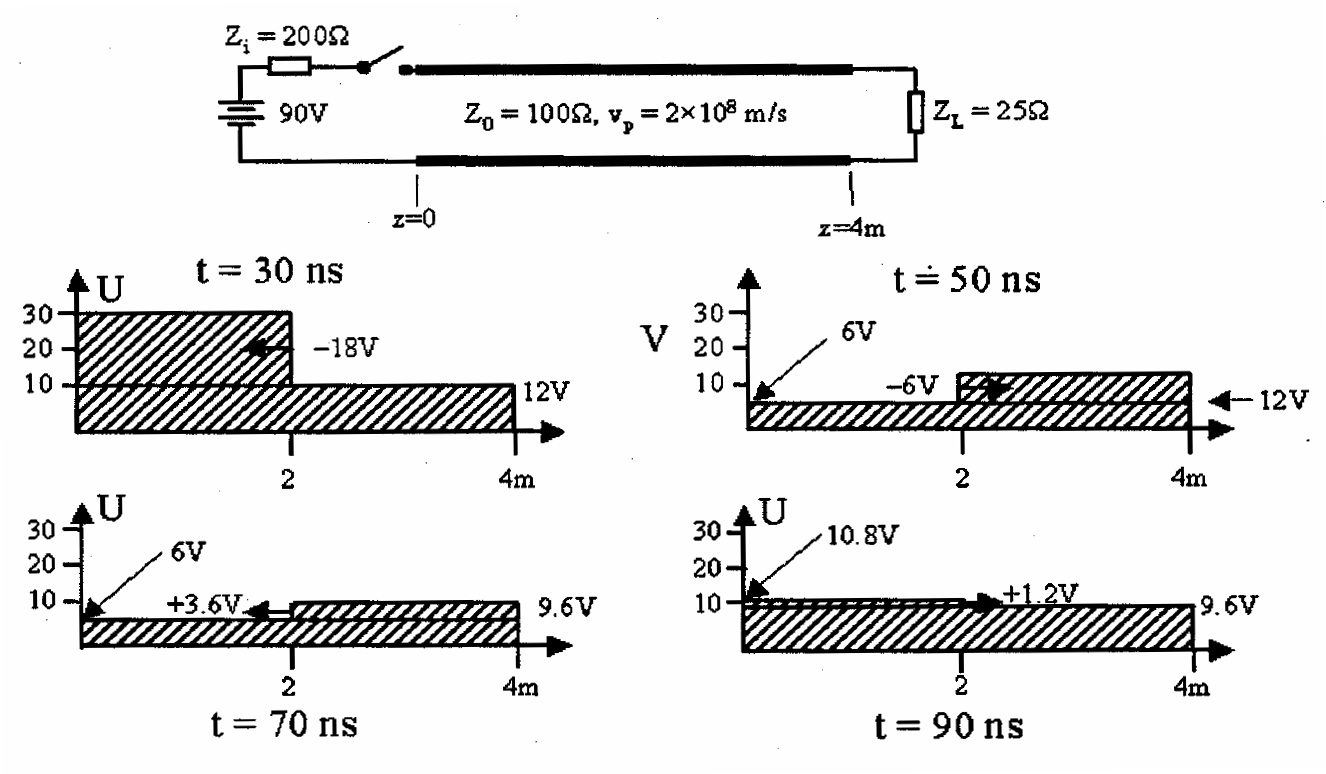
\includegraphics[width=8cm]{./bilder/Leitungen_MFReflx_EnAP_SnAP.png}
%	    \end{minipage}
%		&
%		\begin{minipage}{9cm} 	    	
%    		Das nebenstehende Schema zeigt eine Leitung, welche last- und quellenseitig falsch
%    		abgeschlossen ist. \\
%    		Zur Berechnung der Spannung $\underline{U}_{0}^+$ werden alle Widerstände am Leitungsende
%    		ignoriert ($\underline{Z}_L = 0$).
%    		Die reflektierenden Wellen werden anhand der Reflexionskoeffizienten
%    		$\underline{r}_{Last}, \underline{r}_{Quelle}$ berechnet. Bsp.:
%    		\\ \\
%    		$\underline{U}_{0v} = \frac{U_{Quelle} \underline{Z}_0}{ \underline{Z}_0 +
%    		\underline{Z}_i}; \quad \underline{U}_{r0} = \underline{U}_{v0} \cdot 
%    		\underline{r}_{Last}; \\ \underline{U}_{1}^+ = \underline{U}_{0}^- \cdot 
%    		\underline{\Gamma}_{Quelle}; \quad
%    		\underline{U}_{1}^- = \underline{U}_{1}^+ \cdot 
%    		\underline{\Gamma}_{Last}; \quad$ usw.   \\ 
%    		$\underline{U}_{Resultierend} = \underline{U}_{0}^+ + \underline{U}_{0}^- +
%    		\underline{U}_{1}^+ + \underline{U}_{1}^- +  \ldots  + \underline{U}_{n}^+ +
%    		\underline{U}_{n}^-$
%	    \end{minipage}  
%		\\
%		\begin{minipage}{8cm}  
%			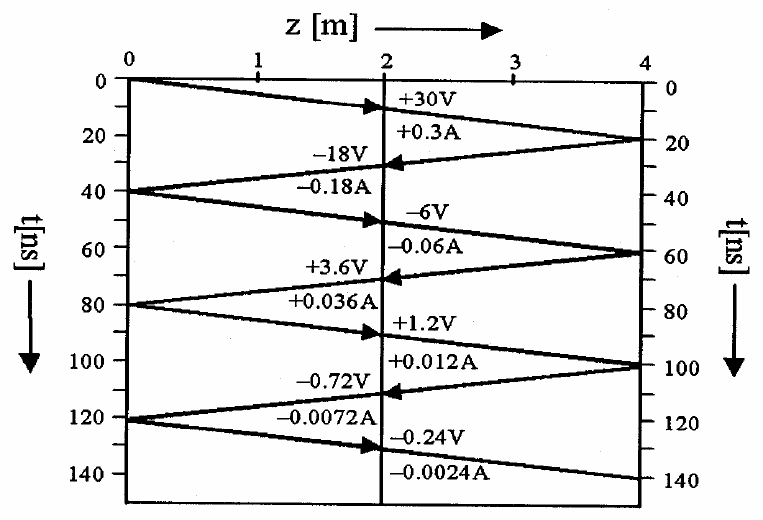
\includegraphics[height=4.1cm]{./bilder/Leitungen_MFReflx_EnAP_SnAP_RaumZeit.png}    	    
%	    \end{minipage}
%		&
%		\begin{minipage}{8cm}
%			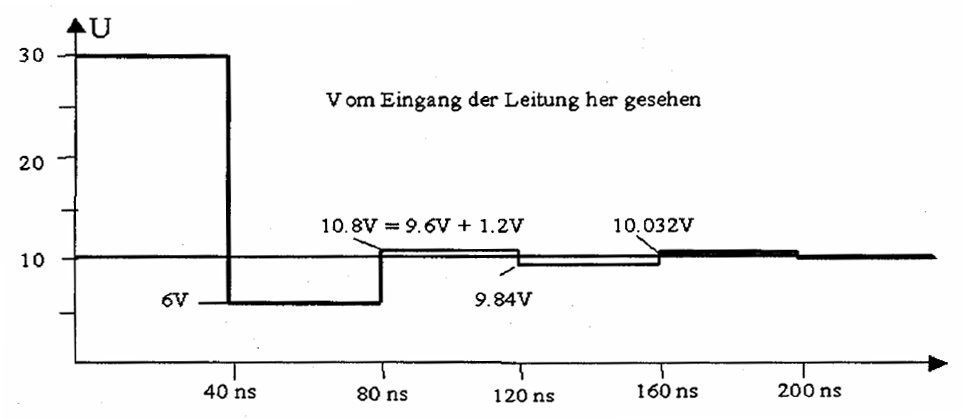
\includegraphics[height=4.1cm]{./bilder/Leitungen_MFReflx_EnAP_SnAP_Eingangsspannung.png}      	
%	    \end{minipage}
%	\end{tabular}

    